\chapter{低級言語で記述した際も実行時間は理論的計算量に従うか}
\section{目的}
本実験の目的は,低級言語で記述したプログラムも,高級言語と同様に実行時間が理論的計算量に従うことを示すことである.今回はアセンブリ言語で記述した選択ソートアルゴリズムを用いて実験を行う.
\section{実験方法}
\ref{fig:実行コマンド}のコマンドで生成したa.outに対し,Linux標準コマンドであるtimeを実行し実行時間を計測する.計測は各ダブルワード列に対して3回行い,その平均を取る.\\
計測された時間をグラフ化する.
ダブルワード列の生成,timeコマンドの実行の仕方は以下に示す.
\begin{lstlisting}[numbers={none}, caption={ダブルワード列の生成(N=データ数)}]
    section .data
data:  times N dd 0
ndata:  equ ($ - data) / 4
\end{lstlisting}
\begin{lstlisting}[numbers={none}, caption={timeの実行(realが実行時間)},label={fig:アセンブリ計測}]
$ time ./a.out
-- 実 行 結 果 ( 略 ) --
real 0m0 .002s
user 0m0 .001s
sys 0m0 .000s
\end{lstlisting}
今回はダブルワードの個数のパターンを1,10,100,1000個までの4つと,1万個から10万個まで1万刻みでの10個,計14パターンとする.

\clearpage

\section{実験結果}
得られた結果を以下に示す.
\begin{figure}[h]
  \begin{minipage}{0.45\textwidth}
  \centering
  \caption{計測結果}
  \begin{tabular}{ll}
    データ個数 & 実行時間\\ \hline
    1 & 0.001\\
    10 & 0.001\\
    100 & 0.002\\
    1,000 & 0.0073\\
    10,000 & 0.1873\\
    20,000 & 0.6077\\
    30,000 & 1.2164\\
    40,000 & 2.0527\\
    50,000 & 2.7173\\
    60,000 & 3.7017\\
    70,000 & 4.8357\\
    80,000 & 5.9860\\
    90,000 & 7.3787\\
    100,000 & 8.8790\\ \hline
  \end{tabular}
  \end{minipage}
  \begin{minipage}{0.45\textwidth}
    \caption{データの個数と実行時間の関係}
    \label{fig:実行時間グラフ}
      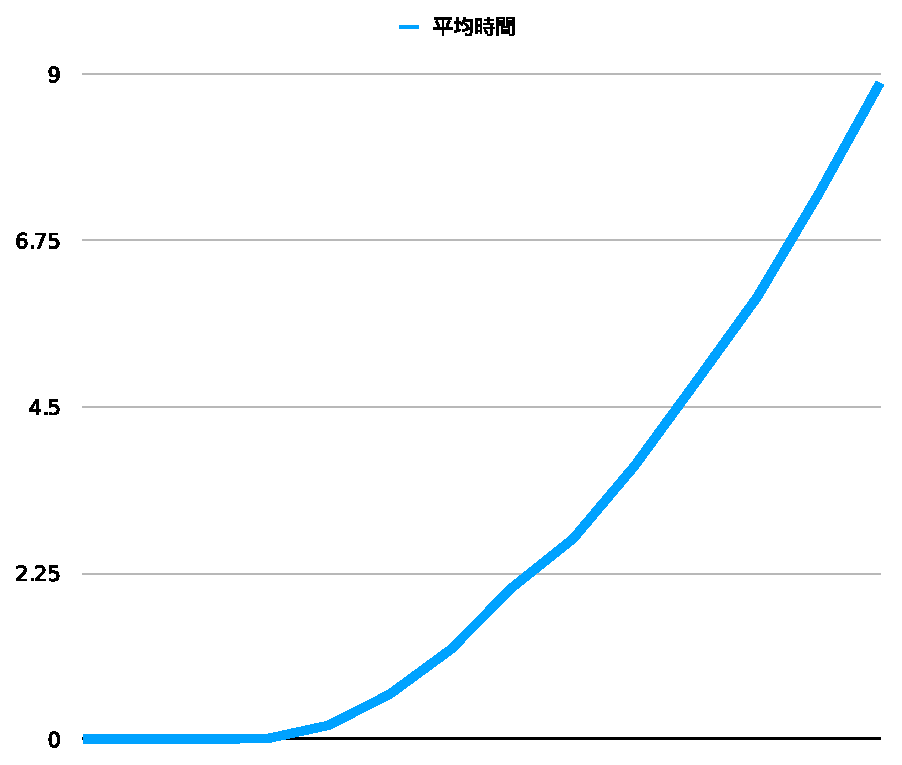
\includegraphics[scale=0.5]{exdata.eps}
    \end{minipage}
\end{figure}

\section{考察}
実験結果の\ref{fig:実行時間グラフ}より,データの個数と実行時間の関係は$n^2$に従っていると考えられる.これは理論的時間計算量である$O(n^2)$の$n^2$と一致するため,アセンブリ言語で直接コードを記述した際もその実行時間は理論的時間計算量に従うと言える.
 \ \ これは,高級言語と低級言語でコードの量に差はあるが,コンピューター内部での処理は同一であるからだろうと考えられる.
